\chapter{Эксперимент CBM на FAIR}\label{sec:secCbm}

% Диссер Ольги Дереновской

% The Compressed Baryonic Matter experiment
% Sélim SEDDIKI
% 10.1051/ epjconf / 201 4 7100120

% http://localhost/Lib/r126c.pdf

Европейский ускорительный центр по исследованию тяжёлых ионов и антипротонов (Facility for Antiproton and Ion Research, FAIR, \cite{FAIR}) создаётся в пригороде Дармштадта в Германии. Это будет исследовательский ускорительный комплекс нового поколения, не имеющий аналогов в мире и открывающий уникальные возможности для проведения научных исследований по наиболее актуальным направлениям современной науки и технологий. Он предоставит высокоэнергетичные, прецизионно настроенные пучки антипротонов и различных ионов от водорода до урана с беспрецедентным качеством и интенсивностью.
%Эти пучки заряженных частиц будут потом ускорены и использованы при создании новых, часто очень экзотических частиц для ряда параллельных экспериментальных программ, одной из которых является плотная барионная материя (Compressed Baryonic Matter, CBM).
Научная программа на ускорительном комплексе FAIR охватывает следующие направления:
\begin{itemize}
\item изучение структуры ядра и исследования в области ядерной астрофизики с использованием пучков стабильных ионов, а также пучков короткоживущих (радиоактивных) ядер, далёких от границы стабильности;
\item изучение структуры адронов, исследования, направленные на развитие и подтверждение теории сильных взаимодействий --- квантовой хромодинамики (КХД), с использованием в основном пучков антипротонов;
\item построение фазовой диаграммы ядерной материи, изучение деконфайнмента кварков и кварк-глюонной плазмы;
\item исследование физики сверхплотной электромагнитной плазмы с использованием интенсивных импульсов пучков тяжёлых ионов в уникальном сочетании с излучением петаваттного лазера;
\item исследования в области атомной физики, квантовой электродинамики в сверхсильных электромагнитных полях с использованием тучков тяжёлых ионов с высокими зарядами и пучков антипротонов;
\item прикладные исследования с пучками ионов для радиационного материаловедения, медицины и биологии.
\end{itemize}

Коллаборации, планирующие исследования на FAIR, разделены на 4 группы:
\begin{itemize}
\item структура ядра и ядерная астрофизика --- NuSTAR (Nuclear STructure, Astrophysics and Reactions);
\item плотная барионная материя --- CBM (Compressed Baryonic Matter);
\item антипротонная программа --- PANDA (antiProton ANnihilation in DArmstadt);
\item физика сверхплотной плазмы, атомная физика, а также прикладные исследования по материаловедению и биологии --- APPA (Atomic, Plasma Physics and Applications).
\end{itemize}

На \figref{fig:FAIRstructure} приведена планируемая схема ускорительного комплекса FAIR рядом с существующей инфраструктурой институтa исследования тяжёлых ионов (Gesellschaft f\"{u}r Schwerionenforschung, GSI).
%FAIR предоставит уникальные возможности для исследования фазовой диаграммы КХД при экстремально высоких плотностях барионной материи наряду с многими другими областями исследований --- адронная физика с антипротоновым пучком, физика ядерных структур с радиоактивным пучком, плазма-физика с высоко-импульсным ядерным пучком.
Центральный элемент комплекса --- двойной синхротрон тяжёлых ионов SIS100/300 (SchwerIonenSynchrotron) длиной 1100~м. В качестве инжектора пучка в SIS100/300 будут выступать существующие в GSI универсальный линейный ускоритель UNILAC (UNIversal Linear ACcelarator) и далее синхротрон SIS18.
Также FAIR включает в себя:
сверхпроводящий магнитный сепаратор фрагментов Super-FRS (Super Fragment Separator),
накопительное кольцо высоких энергий HESR (High Energy Storage Ring),
коллекторное кольцо CR (Collector Ring),
рециркуляционное экспериментальное накопительное кольцо RESR (Recirculation Experimental Storage Ring), 
новое экспериментальное накопительное кольцо NESR (New Experimental Storage Ring),
коплекс для исследования низкоэнергетичных антипротонов и тяжёлых ионов FLAIR (Facility for Low-energy Antiproton and heavy Ion Research).

\begin{figure}[H]
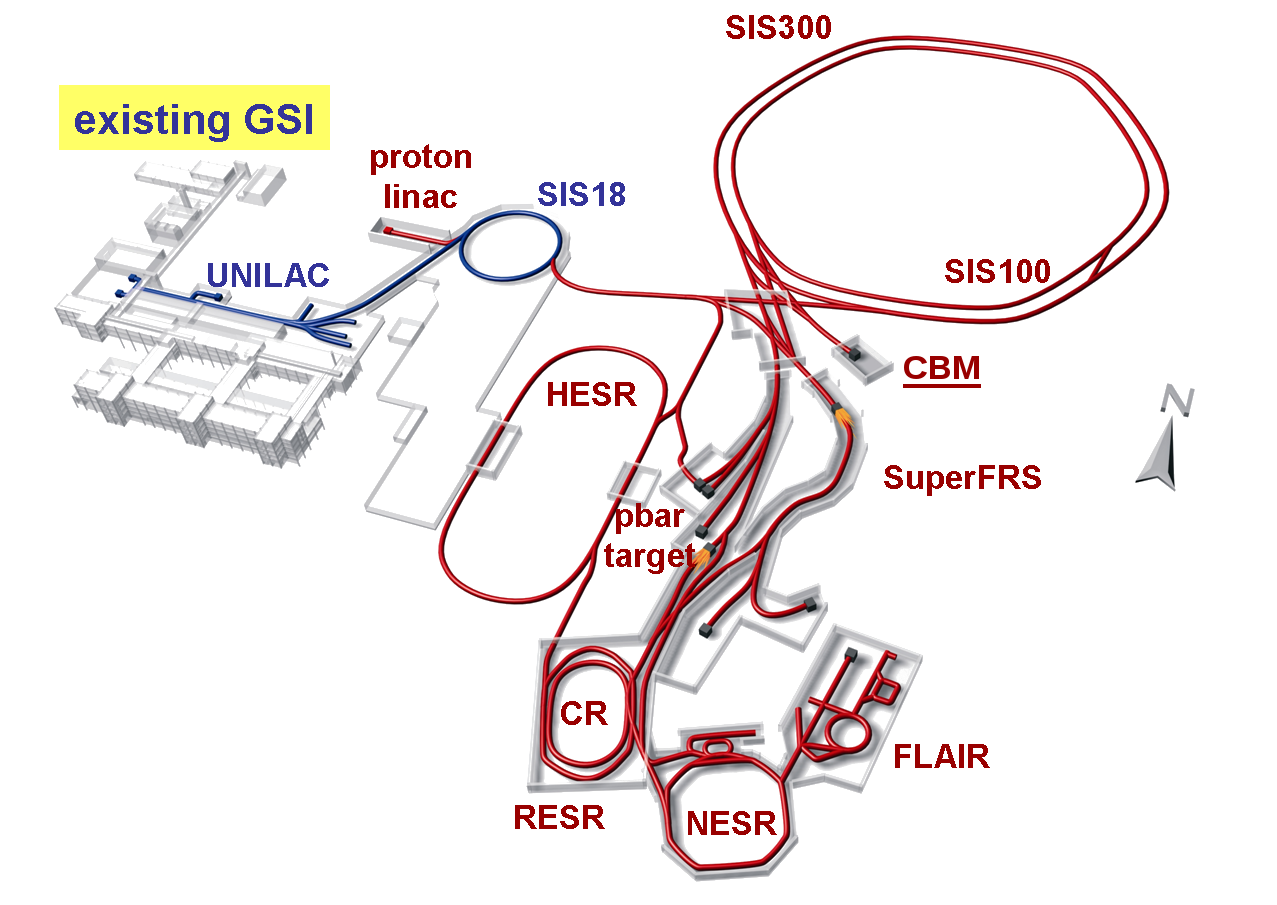
\includegraphics[width=1.0\textwidth]{pictures/FAIR_structure.png}
\caption{Схема FAIR.}
\label{fig:FAIRstructure}
\end{figure}

Для программы ядерных столкновений SIS100/300 предоставит fully stripped \todo пучок, имеющий магнитную жёсткость 100 и 300~мТл соответственно, ионов до урана с очень высокой интенсивнотью (до $2 \times 10^9$ ионов в секунду) и энергией от~2~до~35~\GeVperNucl.
%предоставят лёгкие ионы (Z/A=0.5) будут ускоряться до 45~\GeVperNucl, а протоны --- до 90~\GeV.
Широкий диапазон энергий, предоставляемый FAIR позволит производить ядерную материю при максимальных плотностях, доступных при столкновениях тяжёлых ионов. В соответствии с разными моделями транспорта\todo плотность будет достигать уровня примерно в 12 раз выше обычной плотности барионной материи в ядре и на раннем этапе центрального Au+Au столкновения при энергии пучка 20~\GeVperNucl ($s_{NN} \approx 6.4$~\GeV). \todo \textbf{см. коммент в техе}

%The broad energy range provided by FAIR will allow producing nuclear matter at the maximal net baryon density achievable with heavy ion collisions [8]. As shown in Figure 3, according to various transport models, the density reaches up to about twelve times the normal nuclear matter density in the core and at the early stage of central Au+Au collisions at a beam energy of 20 GeV/nucleon ( (s NN ) ∼ 6.4 GeV). As can be seen in Figure 4, this important feature of the FAIR accelerator is supported by the derived chemical freeze–out parameters that are required to reproduce, within a canonical or grand canonical statistical model, the measured particle yields in central A+A collisions at SIS, AGS, SPS and RHIC energies ( (s NN ) ∼ 2, 5, 20, 200 GeV, respectively) [9]. As the beam energy decreases a clear shift towards lower temperatures and higher μ B occurs.

\todo \textbf{Здесь описать то, как соотносится FAIR с другими ускорителями, на которых выполняются или планируются эксперименты аналогичные CBM. Здесь появляется фазовая диаграмма, LHC, RHIC, NICA. При этом о самих экспериментах, аналогичных CBM, разговор идёт чуть дальше после описания физической программы CBM. Может быть оставить как есть в следующей секции и ничего тут уж не писать?}

Ещё одной отличительной особенностью FAIR являтся то, что он будет предоставлять пучок для нескольких (до~4) исследовательсих установок одновременно, позволяя CBM работать с пучком тяжёлых ионов до 4~месяцев в год. На \figref{fig:FAIRstructure3} показана схема предоставления пучка параллельно нескольким экспериментам.
% Описание можно стырить из FAIR_BTR
Высокая интенсивность пучка и продолжительная его доступность позволят CBM впервые измерять редкие пробы, такие как очарованные адроны и лёгкие векторные мезоны (с помощью дилептонных распадов), в области энергий, предоставляемых FAIR.

\begin{figure}[H]
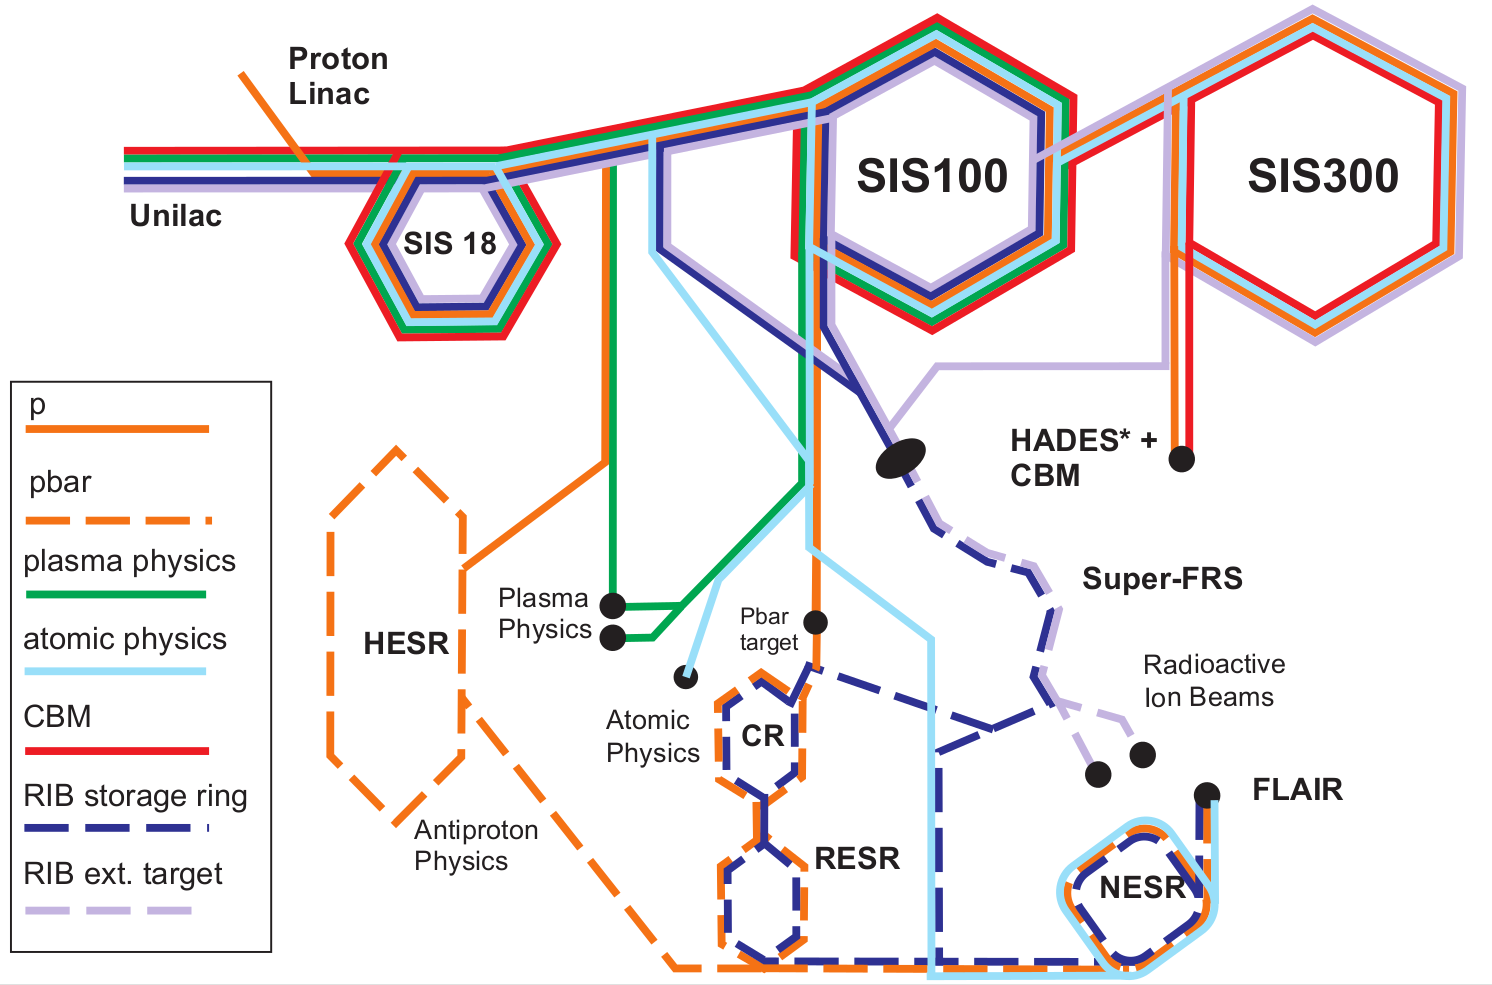
\includegraphics[width=1.0\textwidth]{pictures/FAIR_structure_3.png}
\caption{Схема FAIR.}
\label{fig:FAIRstructure3}
\end{figure}

\section{Физическая программа CBM}

\todo \textbf{Здесь упоминаются эксперименты, аналогичные CBM.}

В отличие от экспериментов в ЦЕРНе и Брукхейвенской национальной лаборатории, где поиск критической точки осуществляется только посредством регистрации спектральных характеристик потоков вторичных частиц (bulk observables), экспериметны FAIR благодаря высокой интенсивности первичных пучков открывают дополнительную возможность регистрировать редкие события со сканированием обширной области фазовой диаграммы по энергиям частиц. В частности планируется впервые непосредственно исследовать сигнатуры (наблюдаемые проявления) возникновения ``огненного шара'' (fireball) --- области ядерной материи, в которой произошёл переход от барионной фазы к кварк-глюонной фазе, --- с помощью регистрации корткоживущих векторных мезонов, распадающихся на дилептонные пары.

Диапазон энергий FAIR 2--35~\GeVperNucl для ионов золота хорошо подходит для проведения экспериментов в области фазовой диаграммы с высокими плотностями ядерной материи, превосходящими нормальную плотность в 8--10 раз.


% https://www.bnl.gov/npp/docs/tribble090712/Vigdor_RHIC_overview_rev2.pdf - слайд 7

RHIC планирует ``даунгрейд'' для выполнения скана по фазовой диаграмме, но \todo всё-равно не заменит FAIR.



\todo \textbf{В разных источниках числа расходятся. Где-то 35, где-то 45...}

Физическая программа CBM нацелена на исследование свойств сверхплотной барионной материи, образующейся в ядро-ядерных столкновениях при энергии пучка от~2~до~45~\GeVperNucl. CBM проектируется с учётом необходимости справляться с измерением высокой статистики адронных, лептонных и фотонных проб в большом аксептансе. Физическая программа включает в себя множество наблюдаемых, среди которых:

\begin{itemize}
\item выход и коллективный поток странных и очарованных адронов; ожидается что они отразят процесс становления деконфайнмента;
\item коллективный поток адронов, который особенно чувствителен к уравнению состояния ядерного вещества на ранних стадиях реакций;
\item производство частиц при пороговых энергиях (странность на SIS100 и очарованность на SIS300), которое может нести важную информацию об уравнении состояний ядерной материи;
\item нестатистические отклонения от события к событию различных параметров (выходы частиц, отношения выходов), связанные с сохранением квантовых чисел (барионных, заряда, странности), которые могут служить сигналом о критической точке КХД;
\item изменение адронных масс в среде, в частности изменение \todo, которые предоставят ценную информацию о внутренних процессах при ожидаемом восстановлении киральной симметрии в плотной барионной материи.
\end{itemize}

\todo \textbf{плоскость реакции - ?}

Экспериментальная задача CBM --- измерять перечисленные наблюдаемые в A+A, p+A, p+p столкновениях как функцию энергии столкновения и размера системы с высокой точностью и статистикой, а также искать нарушения непрерывностей, которые могут служить сигналом о фазовом переходе первого уровня. Данная физическая программа будет выполняться измерением ядерных столкновений при экстремально высоких частотах взаимодействия.

\section{Экспериментальная установка CBM}\label{sec:secCbmSetup}

Для выполнения различных измерений CBM будет функционировать в двух конфигурациях --- с мюонным детектором (MUCH) и с детектором черенковских колец (RICH). Схема экспериментальной установки с RICH представлена на \figref{fig:CBM}.

\begin{figure}[H]
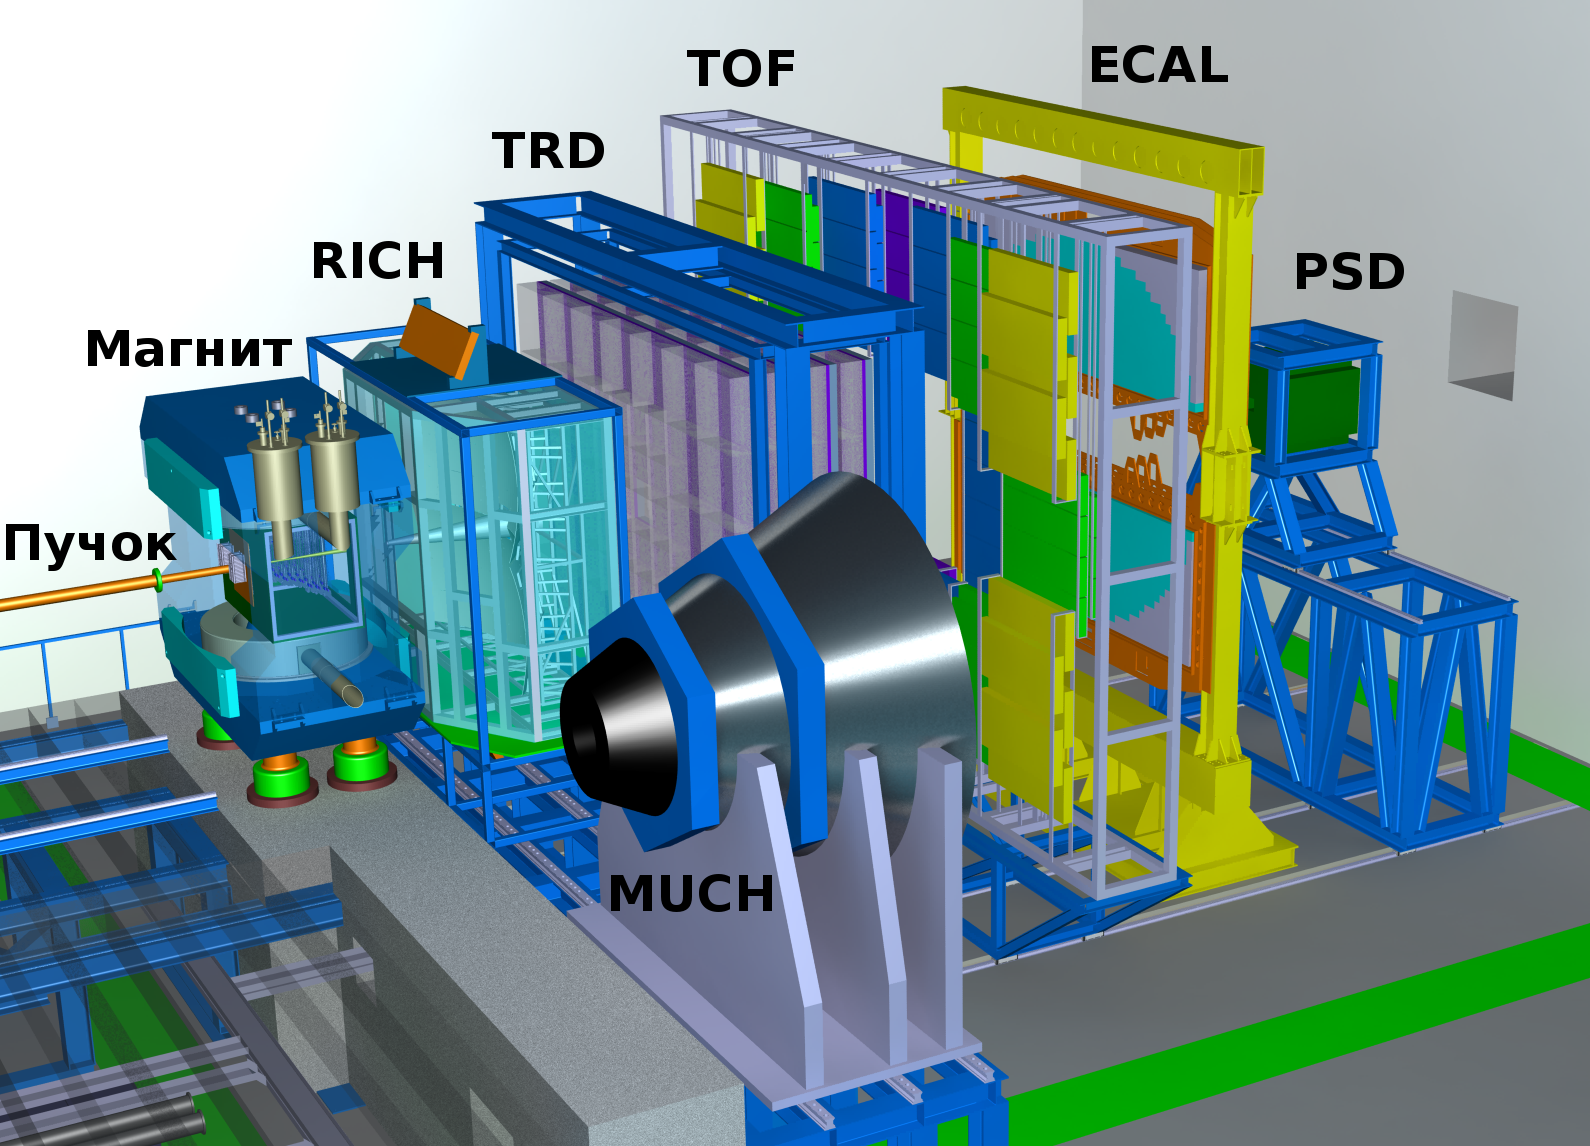
\includegraphics[width=1.0\textwidth]{pictures/1_CBM_SIS100_with_names.png}
\caption{Общий вид экспериментальной установки CBM в конфигурации с RICH.}
\label{fig:CBM}
\end{figure}

Между полюсами сверхпроводящего дипольного магнита~\cite{TDR_Magnet} расположена вакуумная камера, содержащая мишень и вершинный микродетектор (MVD)~\cite{MVD_KOZIEL}, выполненный на основе монолитного пиксельного детектора типа MAPS. Ниже по пучку также между полюсами, но уже вне вакуумной камеры, располагаются станции кремниевой трековой системы (STS)~\cite{TDR_STS}, собранные из двухсторонних микростриповых сенсоров. Координатные трековые детекторы MVD и STS предназначены для реконструкции траекторий заряженных частиц, восстановления их импульсов с точностью не хуже 1\% и нахождения вторичных вершин в условиях высокой множественности и плотности частиц.

Следом за STS в рассматриваемой конфигурации расположен детектор черенковских колец (RICH)~\cite{TDR_RICH}, предназначенный для идентификации электронов и позитронов в диапазоне импульсов от 0.5~\GeVoverC до 8~\GeVoverC с целью восстановления распадов легких векторных мезонов и $ J / \psi $ частиц. Во второй конфигурации на месте RICH стоит мюонная система (MUCH, показана на \figref{fig:CBM} в положении хранения)~\cite{TDR_MUCH}, предназначенная в первую очередь для исследования частиц, распадающихся по димюонному каналу и состоящая из чередующихся слоев железа и газовых трековых камер~\cite{GEM}.

Детектор переходного излучения (TRD) используется для реконструкции треков частиц и идентификации электронов/позитронов в условиях доминирующего фона от пионов~\cite{TRD}. Для идентификации адронов используется время-пролётный детектор (TOF)~\cite{TDR_TOF}. Электромагнитный калориметр (ECAL) типа ``шашлык'' необходим для регистрации прямых фотонов и фотонов от распада нейтральных мезонов ($ \pi^{0}, \eta $)~\cite{ECAL_KOROLKO}. Детектор непровзаимодействовавших осколков ядер (PSD)~\cite{TDR_PSD} представляет собой сегментированный адронный калориметр и служит для определения центральности столкновения и плоскости реакции путем регистрации ядерных осколков, летящих под малыми углами к пучку.

Далее каждый элемент установки описан чуть подробнее.

\subsection{Мишень, вакуумная камера и пучковая труба}\label{sec:secVacChamberPipe}

\subsection{Вершинный микродетектор MVD}\label{sec:secMVD}

\subsection{Кремниевая трекинговая система STS}\label{sec:secSTS}

Задача кремниевой трековой системы --- измерение траекторий и импульсов заряженных частиц, вылетающих из точки взаимодействия пучка тяжёлых ионов с мишенью. Для выполнения физической программы CBM --- наблюдения редких \textbf{явлений} --- необходима частота взаимодействий до 10~МГц, при том что в одном взаимодействии будет рождаться до 1000 заряженных частиц. Реконструкция треков должна выполняться с эффективностью порядка 95\% и разрешением по импульсу порядка $\Delta p / p = 1\%$. Для удовлетворения перечисленных требований STS должна состоять из 8~слоёв кремниевых микростриповых сенсоров, расположенных внутри поля от дипольного магнита на растоянии от 30~см до 100~см от точки взаимодействия вниз по пучку с шагом 10~см.

Сенсоры будут монтироваться на легкую механическую опору в виде карбоновых ферм. Считывание будет осуществляться по многоканальным микро-кабелям самотриггирующейся электроникой, расположенной по краям станций вместе с линиями охлаждения и другими инфраструктурными подсистемами. Микро-кабели будут выполнены из sandwiched polyimide-Aluminum layers толщиной несколько десятков мкм.
%The microstrip sensors will be double-sided with a stereo angle of \SI{7.5}{\degree}
Микростриповые сенсоры будут двухсторонними \todo, шаг между стрипами $58 \mu$м, длина стрипов от 20~до~60~мм, а толщина кремния $300 \mu$м. По текущим оценкам максимальная неионизирующая доза в CBM для сенсоров, расположенных ближе всего к пучку, не будет превышать $10^{14}$ $n_{eq}$ см$^{-2}$. STS будет работать в термостатическом корпусе, обеспечивающем постоянную температуру около \SI{-5}{\degreeCelsius}. Тепло, рассеиваемое считывающей электроникой, отводится с помощью $CO_{2}$ системы охлаждения. Механические опоры детектора и соединения спроектированы так, чтобы была возможность заменить отдельный модуль системы не отсоединяя остальные.

\todo картинка

\subsection{Детектор черенковских колец RICH}\label{sec:secRICH}

\subsection{Мюонная система MUCH}\label{sec:secMUCH}

From CBM MUCH TDR:

The MuCh system is designed to identify muon pairs which are produced in high-energy heavy-ion collisions in the beam energy range from~4~to~40~AGeV. The measurement of lepton pairs is a central part of the CBM research program, as they are very sensitive diagnostic probes of the conditions inside the fireball. At low invariant masses, dileptons provide information on the in-medium modification of vector mesons which is a promising observable for the restoration of chiral symmetry. At intermediate invariant masses, the dilepton spectrum is dominated by thermal radiation from the fireball reflecting its temperature. At invariant masses around $ 3 GeV/c^{2} $, dileptons are the appropriate tool to study the anomalous charmonium suppression in the deconfined phase. In the CBM experiment both electrons and muons will be measured in order to obtain a consistent and comprehensive picture of the dilepton physics.

The experimental challenge for muon measurements in heavy-ion collisions at FAIR energies is to identify low-momentum muons in an environment of high particle densities. The CBM strategy is to track the particles through a hadron absorber system, and to perform a momentum-dependent muon identification. This concept is realized by an instrumented hadron absorber, consisting of staggered absorber plates and tracking stations. The hadron absorbers vary in material and thickness, and the tracking stations consist of detector triplets based on different technologies. The MuCh system is placed downstream of the dipole magnet hosting the Silicon Tracking System (STS) which determines the particle momentum. In order to reduce the number of muons from pion and kaon weak decays, the absorber/detector system has to be as compact as possible.

The MuCh system will be built in stages which are adapted to the beam energies available. Within the FAIR modularized start version the SIS100 ring will provide heavy ion beams with energies up to 14~AGeV, and proton beams up to 29~GeV. The first two versions of MuCh (SIS100-A and SIS100-B) will comprise of~3~and~4 stations suitable for the measurement of low-mass vector mesons in $ A + A $ collisions at 4-6~AGeV and 8-14~AGeV, respectively. The third version of the MuCh system (SIS100-C) will be equipped with an additional iron absorber of 1~m thickness in order to be able to identify charmonium at the highest SIS100 energies. The absorber slices will be built only once so that they could be rearranged properly to obtain required absorber thicknesses. Once SIS300 is operational, we will upgrade the MuCh system further by inserting additional absorbers and detector stations for the measurement of low-mass vector mesons and charmonium at beam energies above 14~AGeV (MuCh versions SIS300-A and SIS300-B).

\subsection{Детектор переходного излучения TRD}\label{sec:secTRD}

\subsection{Время-пролётный детектор TOF}\label{sec:secTOF}

From CBM TOF TDR:

The detector system’s prime task is to measure the arrival time of charged particles to allow for their identification after having matched the TOF - hit with the corresponding STS track obtained from the CBM silicon tracking system (STS). The system is designed to cope with all the reactions anticipated in the physics program of CBM. This ranges from heavy-ion reactions of different system size from C+C to Au+Au over a large incident energy range from 2A GeV to 45A GeV (35A GeV for the heaviest collision system) to proton - nucleus reactions up to a projectile energy of 90 GeV.

Основная задача время-пролётного детектора --- измерять момент времени прихода заряженных частиц, чтобы провести идентификацию после сопоставления хита TOF с соответствующим треком кремниевой трековой системы STS. Детекторная система TOF спроектирована так, чтобы справляться с реакциями, ожидаемыми физической программой CBM. Это подразумевает широкий диапазон взаимодействий от тяжёлых ионов от C+C до Au+Au с энергией от 2A~\GeV до 45A~\GeV до протон-ядерных столкновений с энергией до 90~\GeV.

The general layout considerations following from the CBM concept are discussed in chapter 2.

Since CBM is operated in fixed target mode the flux of charged particles is strongly varying with the polar angle. In order to fit to the forward acceptance of the CBM experimental setup that is based on an instrumented dipole magnet with particle identification detectors placed downstream of the target, a modular TOF wall is proposed whose elements, called modules in the following, are adapted to the granularity and rate requirements. To allow for sufficient separation power especially for the identification of charged kaons, distances of up to 10 m and a system time resolution of 80 ps are necessary leading to an overall size of the TOF - wall of approx. 12$\times$9 m2 . To achieve the overall time resolution this area needs to get instrumented with timing detectors with an intrinsic timing resolution better than 60 ps and an efficiency better than 95\%.

Так как CBM представляет собой эксперимент с фиксированной мишенью, поток заряженных частиц сильн зависит от направления.

Чтобы иметь достаточную степень разделения, особенно для идентификации заряженных каонов, нужно расстояние до 10 м и временное разрешение 80 пс, что приводит к размеру TOF около 12$\times$9 м$^2$. Чтобы достичь необходимого такого временного разрешения детектор должен быть оборудован электроникой с гарантированным временным разрешением лучше 60 пс и эффективностью лучше 95\%.

We propose to build the CBM - TOF wall on the basis of state-of-the-art Multigap Resistive Plate Chambers (MRPC). The basic element of this robust detector concept is a stack of resistive plates made out of glass or ceramics that are separated by thin gas gaps. At sufficiently high electric field strength avalanches are created in a very uniform manner and can be read out via capacitive coupling. As is demonstrated in chapters 7 this 10 - years old detector technology is well advanced by now, largely due to the effort of the CBM - TOF group, and offers the flexibility to cope with the high demands posed by the CBM physics goals. Most notably, the proposed concept that requires a detector technology with a sustained rate capability in the order of 25 kHz/cm 2 became possible only by the development of a low - resistivity glass (see section 7.1.1) that is available for CBM - TOF by now through the CBM - TOF group at Tsinghua University, Beijing, China at reasonable costs.

Предлагается построить CBM TOF на основе современных MRPC. Базовый элемент этого robust детектора --- пачка резистивных пластин из стекла или керамики, которые разделены тонким зазором с газом. При достаточно высоком электрическом поле создаются очень равномерные ливни, которые можно считывать с помощью capacitive coupling.

The proposed structure of the CBM - TOF wall is based on detector layouts that have already been
realized and tested in in-beam experiments and demonstrated MRPC counter timing resolutions below
60 ps with efficiencies above 95\% at rates relevant for CBM (see chapter 7 for details). The basic element
of the proposed wall are MRPC strip counters where a single avalanche is generating two signals at
the two ends of a readout-electrode. The length of the readout - strip can be easily adjusted to the
required granularity. The leading design goal of the proposed strip structures is operation stability and
signal integrity. This is achieved by differential signal processing and the matching of the readout strip
impedance to the input impedance of the newly developed preamplifier discriminator chip (PADI). Thus
the number of spurious hits due to reflections is minimized and an optimal response of the detectors is
guaranteed with minimal dead time. This aspect is considered to be especially important for the high
rate running conditions of CBM where even independent events will be overlapping in time space and
any additional spurious hit will deteriorate the system performance.

In order to minimize the number of components, the CBM - TOF wall is designed to be composed of
only 4 different types of MRPC counters, arranged into 6 different types of modules. The proposed CBM
-TOF system is described in detail in chapter 3.
The modules and counters are realized in 2 different technologies:
1. The modules placed at small polar angles close to the beampipe (M1 - M3) are housing counters
(MRPC1,MRPC2) that employ a double stack HV - design. The counters are equipped with low
resistivity glass and have electrodes of 32$\times$10 cm 2 and 32$\times$20 cm 2 dimensions, 10 gas gaps and a
strip pitch of 4.7 mm. The front-end electronics is mounted outside of the gas volume. A total of
36.608 electronics channels is needed to readout this part of the TOF wall.
The proposed design emphasize the full coverage of the solid angle and is rather conservative in
terms of data integrity since each hit is registered by 2 readout channels and allows to determine
the hit position with an accuracy of a few mm in each direction.
More detailed measurements of the response under fully loaded conditions and time based simula-
tions of the system response will show whether this strip solution could be replaced by a cheaper
pad - type MRPC solution that is described in detail in the appendix E and requires only 27.792
electronic readout channels.
A decision will be taken at latest in Dec. 2015 after careful analysis of test beam data that will
be taken at GSI in October 2014 and at CERN SPS in April 2015. With currently available HI -
beam, conditions close to the operating conditions of CBM will be realized.
2. For the remaining part of the wall (modules M4 - M6) two different sizes of a MRPC strip counter
with active area of 32$\times$27 cm 2 and 32$\times$53 cm 2 , and a strip pitch of 1 cm are proposed. These
counters are equipped with low - resistivity glass or thin float glass electrodes according to the rate
requirements and use a single HV stack with 8 gas gaps. In order to optimize the signal integrity
the preamplifier is connected as directly as possible to the readout electrode and put into the gas
volume of the modules. As largest benefit this arrangement offers the possibility to operate the
detectors at lower discriminator thresholds and the lower pulse height results in turn also in a higher
rate capability. The design of independent module units including the analog electronics also offers
the necessary robustness to operate a system of 218 modules and 70.000 readout channels.
The disadvantage of the proposed single stack architecture is the need of two high voltages ($\pm$11 kV)
causing substantial costs. An alternate design with a double stack configuration of the high voltage
is available and can be operated at about 5.6 kV. However, this counter configuration needs more
glass electrodes (12 instead of 9) and the cost benefit from the HV has to be compared to the
additional cost caused by additional electrodes especially when these are made from low resistivity
glass. Counters of this type that are described in appendix F.2.4 will be evaluated in comparison to
the proposed ones also in the upcoming HI - test beam campaigns addressing the system features of
the designs. A decision will be taken at latest in Dec. 2015 after careful analysis of the test beam
data.
The high performance electronics for the whole CBM - TOF wall is independent of the choice of a specific
module or counter type and is based on the PADI and the GET4 - ASIC chips developed by the CBM -
TOF group (see sections 3.3.3 and 3.3.5). The combination of both chips in conjunction with a custom -
designed clock distribution system (section 3.3.8) offers the possibility to build a large scale system with
an electronics contribution to the timing resolution of about 30 ps. This system was tested using a readout
controller that implements the full CBMnet - protocol and allows for online inspection and control of the
GET4 - data. The details of the readout-chain are described in section 3.3.
However, since up to now no long - term stably working GET4 - system could be demonstrated, an al-
ternative backup solution is also included in this report. It is built on FPGA based TDCs that became
available recently (see appendix G.2) and provides timing resolution on the level of 10 ps. A free - stream-
ing readout chain is not yet available, but is planned to be realized in the near future. As a consequence
the number of necessary readout controllers would be substantially reduced leading eventually to a more
simple and cost effective system. More R'n'D is required in the direction of an FPGA - based digitizer /
readout system, specifically considering the radiation environment (see chapter 2.5).
Since FPGA - based digitizers are offering a better resolution and more flexibility and would allow e.g.
for an improvement of the double hit recognition the decision about the production of the GET4 - system
will be taken only after a) the stability of the GET4 readout chain is proven, b) no competitive FPGA
based solution is available until start of mass production (Dec.2015). Therefore R'n'D work on FPGA -
based TDCs is continuing as part of the project.
The proposal of a high performance TOF wall would be incomplete without the discussion of the time
- zero (T 0 ) - reference that is needed for any velocity measurement. Details can be found in chapter 4
demonstrating that for all of the anticipated running scenarios solutions are available. For most of the
heavy-ion reaction running at the initial SIS100 accelerator the software based T 0 - extraction is sufficient
(see section 4.2). This method can be calibrated by making use of the diamond based start detector
system developed for the HADES experiment (section 4.4) that is operational up to interaction rates of
100 kHz.
As has been shown by Monte-Carlo simulations using the SHIELD event generator the quality of the T 0
- reference determination can be improved by installing the so called Beam Fragmentation T 0 Counter
(BFTC) as the innermost part of the TOF wall (see section 4.3). It should cover the region from about
20 to 60 cm from the beam pipe (overlapping with the PSD acceptance). Using a very simple algorithm
without tracking information a T 0 - signal with a precision of better than 50 ps can be achieved. A detector
concept, anticipated to be able to operate in this harsh environment with fluxes being as high as 100
kHz/cm 2 , built from very radiation-hard materials and possessing minimum gas aging characteristics, is
suggested to be based on the ceramic electrodes (see section F.1). Single cell pads with the size of 2$\times$2
cm 2 seem to fulfill the double hit, maximum rate and cross-talks requirements. Further R'n'D is necessary
in order to prove the validity of the concept.
The very large dynamical range in terms of incident beam energies that has to be covered by the CBM
experiment reflects itself by the movable wall concept where the whole TOF - system is mounted on rails
and can be placed at various distances. The rail system is sketched in section 5.1. It allows e.g. to
balance the decay losses for kaons against the purity of an anticipated online kaon multiplicity selection.
It also enables the servicing of the components independently from the other subsystems of CBM during
shutdown periods.

\subsection{Электромагнитный калориметр ECAL}\label{sec:secECAL}

\subsection{Детектор PSD}\label{sec:secPSD}

\section{CBM RICH поподробней}

\todo \textbf{Может как-то сделать так, чтобы это описание CBM рича было после описания других ричей --- COMPASS, LHCb, HERA-b? Или как раз наоборот, лучше сразу после этой секции?}

\todo \textbf{Перенести какую-то часть из секции RICHgeo}

Особенность CBM RICH заключается в том, что в плоскости реконструкции одновременно необходимо восстанавливать порядка \todo колец. 
\todo хитов в плоскости реконструкции, из них \todo сигнальных, а остальные шумовые (откуда\todo  конверсия в материале до рича\todo , \todo хитов на кольцо, \todo колец от пионов, \todo колец от электронов, \todo колец от \todo

\todo \textbf{далее параметры реконструкции и какие-то слова о том, как это соотносится с другими ричами.}
